% This is LLNCS.DOC the documentation file of
% the LaTeX2e class from Springer-Verlag
% for Lecture Notes in Computer Science, version 2.4
\documentclass{llncs}
\usepackage{llncsdoc}
\usepackage{graphicx}
\usepackage{hyperref}
%
\begin{document}
%\markboth{\LaTeXe{} Class for Lecture Notes in Computer
%Science}{\LaTeXe{} Class for Lecture Notes in Computer Science}
%\thispagestyle{empty}
%\begin{flushleft}
%\LARGE\bfseries Instructions for Authors\\
%Coding with \LaTeX\\[2cm]
%\end{flushleft}
%\rule{\textwidth}{1pt}
%\vspace{2pt}
%\begin{flushright}
%\Huge
%\begin{tabular}{@{}l}
%\LaTeXe{} Class\\
%for Lecture Notes\\
%in Computer Science\\[6pt]
%{\Large Version 2.4}
%\end{tabular}
%\end{flushright}
%\rule{\textwidth}{1pt}
%\vfill

%\begin{flushleft}
%\large\itshape
%\begin{tabular}{@{}l}
%{\Large\upshape\bfseries Springer}\\[8pt]
%Berlin\enspace Heidelberg\enspace New\kern0.1em York\\[5pt]
%Barcelona\enspace Budapest\enspace Hong\kern0.2em Kong\\[5pt]
%London\enspace Milan\enspace Paris\enspace\\[5pt]
%Santa\kern0.2em Clara\enspace Singapore\enspace Tokyo
%\end{tabular}
%\end{flushleft}
\newpage
%
%\section*{For further information please contact us:}
%%
%\begin{flushleft}
%\begin{tabular}{l@{\quad}l@{\hspace{3mm}}l@{\qquad}l}
%$\bullet$&\multicolumn{3}{@{}l}{\bfseries LNCS Editorial Office}\\[1mm]
%&\multicolumn{3}{@{}l}{Springer-Verlag}\\
%&\multicolumn{3}{@{}l}{Computer Science Editorial}\\
%&\multicolumn{3}{@{}l}{Tiergartenstra�e 17}\\
%&\multicolumn{3}{@{}l}{69121 Heidelberg}\\
%&\multicolumn{3}{@{}l}{Germany}\\[0.5mm]
% & Tel:       & +49-6221-487-8706\\
% & Fax:       & +49-6221-487-8588\\
% & e-mail:    & \tt lncs@springer.com    & for editorial questions\\
% &            & \tt texhelp@springer.de & for \TeX{} problems\\[2mm]
%\noalign{\rule{\textwidth}{1pt}}
%\noalign{\vskip2mm}
%%
%%{\tt svserv@vax.ntp.springer.de}\hfil first try the \verb|help|
%%command.
%%
%$\bullet$&\multicolumn{3}{@{}l}{\bfseries We are also reachable through the world wide web:}\\[1mm]
%         &\multicolumn{2}{@{}l}{\texttt{http://www.springer.com}}&Springer Global Website\\
%         &\multicolumn{2}{@{}l}{\texttt{http://www.springer.com/lncs}}&LNCS home page\\
%         &\multicolumn{2}{@{}l}{\texttt{http://www.springerlink.com}}&data repository\\
%         &\multicolumn{2}{@{}l}{\texttt{ftp://ftp.springer.de}}&FTP server
%\end{tabular}
%\end{flushleft}


%
%\newpage
%\tableofcontents
%\newpage
%

\title{Using ANN learning to solve Ludo as a blackbox problem}
\author{Frederik Hagelskjaer}
\institute{University of Southern Denmark, Campusvej 55, 5230 Odense M, Denmark \\frhag10@student.sdu.dk}
\maketitle

\begin{abstract}

This article is the hand in for the course AI2 at the University of Southern Denmark. It concerns the training of a neural network for playing ludo. The approach is a black box approach were the algorithm is to be trained without using any prior analysis of the ludo game. Thus the goal is to analyse the abilities of using simple training with backpropagation using moves from good LUDO players. Thus the state of the board is used without any preprocessing. It is shown that normal learning algorithms are not able to cope with the complexity of LUDO. Backpropagation trying to learn from players using GOFAI cannot simply learn. It is concluded that preprocessing of data is an important aspect in learning algorithms. An interesting aspect found is that most neural networks initiated with random parameters will outperform a random player significantly. 

\end{abstract}

\section*{Introduction} % 5


%The LUDO game. 
%Using AI to develop a Ludo playing agent. 
%There are no real requirements to the agents performance, but the results of the developed AI should be extensively documented. 
%The goal of AI is an introduction to artificial neural networks, and therefore the agents developed in this article will use such an approach.


The idea for this article is to understand the limits of using artificial neural networks, ANN, to solve problems. Thus it is not the goal to simply create the LUDO player with the best performance, but to understand how the performance depends on the development of the network. 

The complexity of the LUDO game, makes it impossible to make a analytical solution by simply creating a lookup table with every solution for every state, thus making decision making a lookup table, as shown in \cite{6031999}. This article tries to determine an appropriate neural network for an agent playing on level with other solutions.

The performance of the ludo player will be measured by the proverb: "If you ain't first you're last" \footnote{ $http://en.wikiquote.org/wiki/Talladega\_Nights:\_The\_Ballad\_of\_Ricky\_Bobby$}
, thus only the amount of victories will be measured. That is test will be run for the ludo player against proportional opponents until a linearity is found, i.e. more plays wont change the relationship between wins.

%Tweaking of input could also be called embodied AI, move when pushed or something.

The goal will be to avoid any "tweaking" of parameters towards the creation of the neural network. Examples of such tweaking will be shown, both to show it's strengths and why it is desirable to avoid. Neural networks are often created with preprocessed input \cite{NeuronOnline}. 

An example of such preprocessing can be seen by looking at the ludo game and it's dynamics. Every turn a piece is dictated to move forward, and except from stars and globes overall progress is the same. Thus one could speculate that the most important factor is hitting home. One could thus give the relationship  of positions between pieces instead of all positions, as seen in figure %\ref{?}. 

%Several methods exist to form


%The indicating the gain from using stars and globes.


The problem is that this isn't necessarily the best solution and could thus steer the network towards a suboptimal solution. Thus the idea is to create neural networks trained only by the knowledge that winning is positive. Seeing ludo as a black box problem. 


\section*{The neural network} % 40%


The neural networks were implemented using PyBrain described in \cite{schaul2010}. This was done because of a desire to obtain the flexibility and ease of Python while still retaining the speed of C. 

The implementation of the ludo game was done using Leon Larsens ludosimulator.

Before training the neural networks the dimension of the neural network must be decided. There exist no formal definition for how to chose the size of a network with unknown complexity. Though to avoid over fitting the system when training, the dimension should not be to large. A standard element of neural networks is the perceptron taking weighted input and returns 0 or 1. Thus a combination of these could decide which brick to move. The problem is that a single layer perceptron is a linear separator and to avoid this a hidden layer is introduced \cite{Russell}.

The ludo player developed uses a neural network to decide which brick to move given state and roll values. The values are scaled between 0 and 1 . In ludo one cannot decide not to move any of the bricks and thus it necessary to guarantee that the move is legal. This is done by taking the best value that gives a change in states and using that as the move. The start position is a random start value, so if all ranks were equal it would be a random output.

The number of and size of the hidden layers will be described in each test, though input and output size stays the same.

To train the network towards the optimal multiple procedures were explored. These methods are described in the following section.

\section*{Imitating Human Player}
 

Originally neural networks were trained using different error minimization procedures. 
Back-propagating was used.

\subsection*{Methods}


Thus it is necessary to provide a training signal for this approach. By looking at different ludo games and measuring the procedure of the winner one could create train a neuron to make winner decisions. The system is still seen as a black box as no evaluation is done on the actual moves, they are simply used by the winner.

As no data set of ludo winner moves were available an imitation were performed. Test data were collected by agents taking random moves playing against each other. By a chance of 1/200 the board state and dice roll were added to a dataset. 

A test person then evaluates the data, and chose the "perceived" optimal move. Thus a learning set were created for the back propagation algorithm.

The first test is to see whether it is possible to train a neural network using datasets with an answers provided by a human. More than 200 situations were evaluated before before the training began. Using pack-propagation the neural network were trained to fit the data set, and made to play against opponent. 


Backpropagation method.

For the backpropagation method the data set were split into a training and test set with a proportion of 0.25. 


The training data for the human player can be found on Dropbox  \footnote{ \url{https://www.dropbox.com/s/i3fa0ewf9xxtyy5/marius_list_scaled.dat}}, it consist of 237 states with 17 input and 1 output scaled between 0 and 1, as a PyBrain ClassificationDataSet.

\subsection*{Results}

Figure \ref{fig:ligener} shows the result of 1000 games of LUDO against three random players. The neural network is able to win with a small margin.  

\begin{figure}[t]
        \centering
		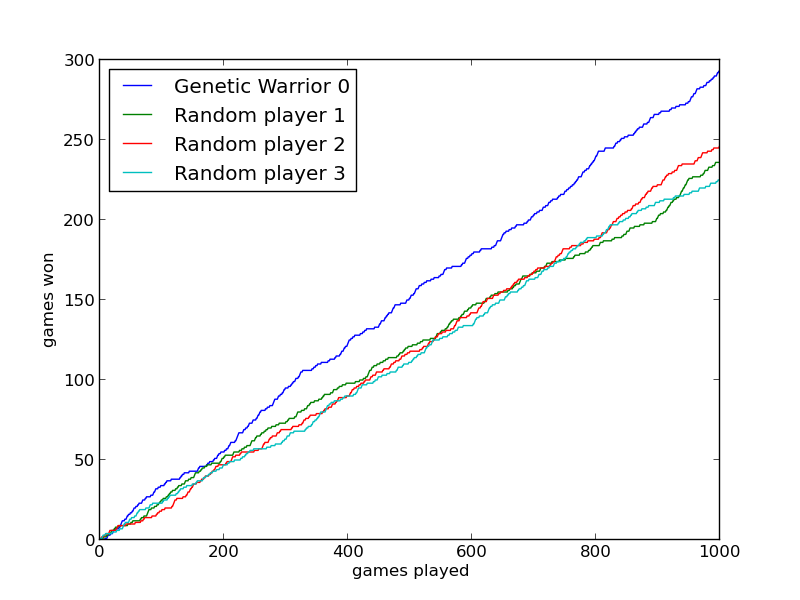
\includegraphics[scale=0.3]{../lillens_gener_unscaled_u.png} 
        \caption{ Result of 1000 ludo games. Genetic warrior being the trained neural network.}\label{fig:ligener}
\end{figure} 

Training error should be included.


\subsection*{Analysis and Discussion}

It is shown that it is possible to train a network to be able to beat the opponent. 

Very hard works better

Makes sense

\section*{Randomly Winning}

Another test were performed to test the pack propagations possibility of learning simply from random games. Numerous games were played with random agents and for every game that resulted in a win, states chosen moveer were collected for every round. Thus a dataset to win against random agents were created. 

\subsection*{Method} 

To test what network best fitted such data, backpropagation were  performed for increasingly larger neural network with along with an increasing number of training epochs. Using this data a player was created to compete against random players.

\subsection*{Result}

The test for lowest error can be seen in figure 


Fitting the data using automatically generated data. Trying to decide the optimal size to fit the data, i.e. the test data.

\begin{figure}[t]
        \centering
		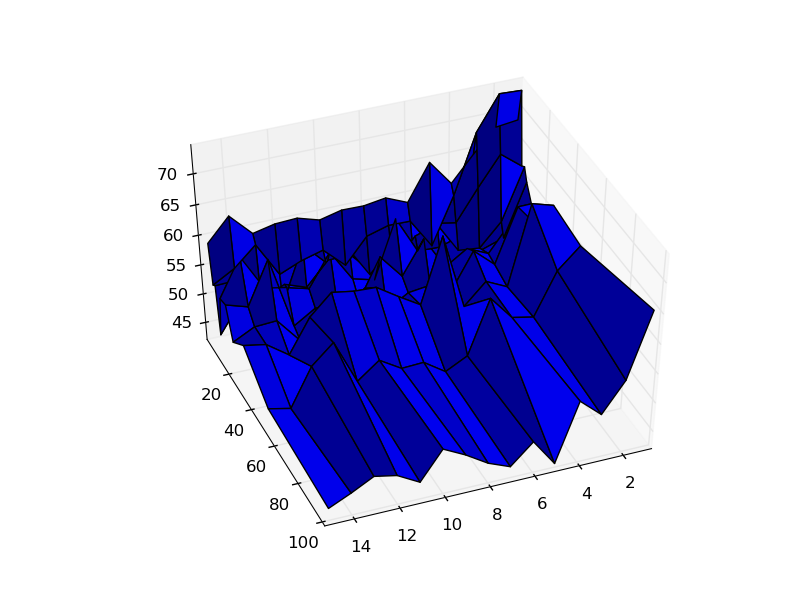
\includegraphics[scale=0.3]{../testing_fit_3D.png} 
        \caption{ Plot showing the error of the training set using different epochs and number of hidden neurons. Respectively on the right and left side.}\label{fig:3D}
\end{figure} 



\subsection*{Analysis and Discussion}



\section*{Imitating Another Agent}

The ran


As it didn't g



\section*{Random Neural Networks}

A test were performed to check the performance of neural networks with randomly generated parameters. The test was done to check the effectiveness of the training.

\subsection*{Method}

It was seen that the trained networks did perform better than the random players. Though to test that this is actually the result of training, the effectiveness of simply using neural networks are to be tested. Randomly generated parameters between -1 and 1. The network was made with a hidden layer of size 5 with no bias. 50 different neural networks playing against three random players. 

\subsection*{Results}

The results of the multiple agents games can be seen in figure \ref{fig:random_50}. Only in one of the games is the number of wins less than 25. The mean of multiple of such simulations never went below 40 wins.

\begin{figure}[t]
        \centering
		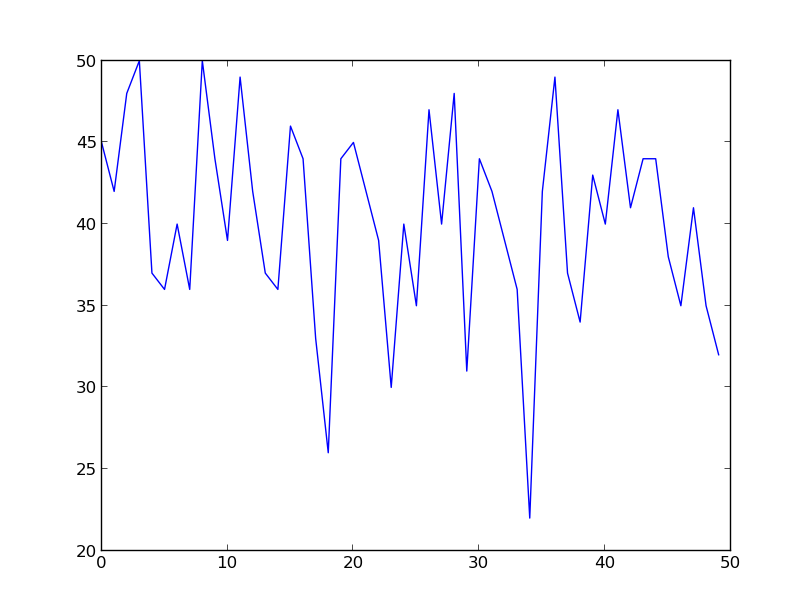
\includegraphics[scale=0.3]{../50_random_1.png} 
        \caption{ Number of wins for 100 ludo games for 50 different randomly generated neural networks. }\label{fig:random_50}
\end{figure} 

\subsection*{Analysis and Discussion}

It can be seen simply having a plan makes the network better. It is possible that the scaling of inputs between  -1 and 1 did have and effect in making the parameters good.

Most likely it simply stems from the fact that moving more consistently, when possible is a better strategy than moving random.


\section*{Playing against other Agents}

It makes sense that it is very hard to fit acutally some of random players .

Leons agent. Trained seequntially with preprocessed input.

\section*{Results} % 20%


By using the trained data from the human choices the following results were found.


Figures.






For the genetic algorithm multiple randomly generated parameters were created.

\subsection*{Random Data}

Random data results. All neural networks outperform the random players. Data set, example.
The results from such a test involving 50 different networks can be seen in figure \ref{fig:random_50}.



Analysis of moves actually being used.

%30 \tilde{ } 50

No immediate connection were seen between the sound and good moves.



\section*{Analysis and Discussion} % 25%

From the initial generation of datasets with random parameters it can be seen that all most all of them outperform the random approach. This indicates that using somewhat of a plan will outperform a completely random approach, expect of course if the plan is 


Look into grouping of whether certain moves belong to a "winning" or losing set.



\section*{Conclusion} % 5%

Conclusive  works better than random, almost 

Very complicated when using complete board as input.

Training towards other players - what are the results.


Instead one should look into the problem. Properly solve the small problems first.  


\section*{Acknowledgements} %5

Marius Hagelskjaer, my little brother, for sitting through and judging more than 200 different ludo states. \\

\noindent Leon Larsen, for providing the sequential LUDO player to play against. \\

\noindent The simulator was developed in shared effort with Kent Stark Olsen, Rudi Hansen and Frederik Hagelskjaer.

\begin{thebibliography}{[MT1]}
%

\bibitem[IC]{NeuronOnline}
\url{http://www.doc.ic.ac.uk/~nd/surprise_96/journal/vol4/cs11/report.html}
May (2014)
%

\bibitem[AI2]{Russell}
Russell, Stuart J., Norvig, Peter
Artificial Intelligence: A Modern Approach
2. Edition
Pearson Education (2010)
%
\bibitem[SR1]{schaul2010}
Schaul, Tom and Bayer, Justin and Wierstra, Daan and Sun, Yi and Felder, Martin and Sehnke, Frank and R\"{u}ckstie\ss, Thomas and Schmidhuber, J\"{u}rgen
PyBrain
Journal of Machine Learning Research (2010)
%
\bibitem[DR1]{Rumelhart}
Rumelhart, David E. and Hinton, Geoffrey E. and Williams, Ronald J.
Learning Representations by Back-propagating Errors
Neurocomputing: Foundations of Research 696--699 (1988)
%
\bibitem[FA1]{ludoanalysis}
Alvi, F. and Ahmed, M.
Complexity analysis and playing strategies for Ludo and its variant race games
Computational Intelligence and Games (CIG), 2011 IEEE Conference on 134-141 (2011)
%
\bibitem[FM1]{frean:mar}
Frean, Marcus
The upstart algorithm: A method for constructing and training feedforward neural networks
Neural Computation 2, 198-209 (1990)
%


\end{thebibliography}


\end{document}
